 %%%%%%%%%%%%%%%%
 % Useful stuff %
 %%%%%%%%%%%%%%%%
\renewcommand{\vec}[1]{\ensuremath{\mathbf #1}}

\subsection*{The governing equation}
\todo[inline]{from helluy's doc}
The transmission model line is given by the following system of differential equations
\begin{equation}
  \label{eq:model}
    \begin{array}{ccc}
      \partial_z U&=& L\partial_t I + RI \\
      \partial_z I&=& C\partial_t U + GU \\
    \end{array}
\end{equation}

where we denoted the following square matrices:
\begin{itemize}
\item  $L$ the inductance, required to be \textbf{definite-positive and symmetric}
\item $C$ the capacity, defined as the inverse of $L$, required to be \textbf{definite positive and symmetric}
\item $R$ the resistance\todo{pas sur du mot}, assumed to be diagonal
\item $G$ the conductancy, defined as the inverse of $R$.
\end{itemize}

we get rid \todo{change this} of the time dependancy in $\eqref{eq:model}$ by
applying a Fourier transformation $(U,I) \mapsto (\hat{U},\hat{I})$, one
finally gets, after dropping the hats the following system
\begin{equation}
  \label{eq:model.fourier}
    \begin{array}{ccc}
      \partial_z U &=& (j\omega L + R) I \\
      \partial_z I &=& (j\omega C  + G) U \\  
    \end{array}
\end{equation}
for the latter we denote by $Z$ the impedance matrix defined by $Z=(j\omega L +
R)$ and $Y=(j\omega C  + G)$. The main concern of this paper is to compute $L$
with desired properties, independantly \todo{ ? } from the number of
conductors, $C$ is straightforwardly deduced.

In the following chapters, we give the steps to compute the matrices at the
continuous scale. We then suggest a way to enforce the symmetry and the
definite positive conditions.
\subsection*{The single armour case}
\todo[inline]{rewrite from helluy's doc all the blabla}
In what follows we derive the expression of $C$ in the case of one armour $w_0$
containing $N$ cables $\{ w_i \}_{i=1,...,N}$. We assume that the magnetic
field $\vec{B}$ derives from a potential field $\vec{A}=(0,0,\varphi(x,y))$
such that 
\[
\label{def:B}
\vec{B} = \rot  \vec{A}
\]

We focus on every $w_i$ inside $w_0$, the latter definiton combined with
Maxwell-flux equation $\rot \vec{B} = \vec{j}$ on $w_i$ leads to a Poisson-like
equation satisfied by $\varphi$ on $w_i$,

\begin{equation}
\label{eq:poissonwi}
\rot \vec{B} = -\Delta \varphi = j_z \quad \text{on } w_i
\end{equation}

Since $\varphi$ is assumed regular enough, one can use the Gauss identity to infer
\begin{equation}
  \label{eq:traceeqn}
  \begin{array}{rcl}
    \int_{w_i} (-\Delta \varphi) \, dV &=& \int_{w_i} (- \divg (\nabla \varphi))  dV \\
                                       &=& \int_{\partial w_i} (-\nabla\varphi \cdot \vec{n}) dS \\
                                       &=& \int_{\partial w_i} \nabla\varphi \cdot (-\vec{n})  \, dS \\
                                       &=& \int_{ \partial w_i} \nabla\varphi^{\text{ext}} \cdot (\vec{n}_i)  \, dS \\
                                       &=& I_i \\
  \end{array}
\end{equation}
where $\vec{n}_i$ denotes the normal vector pointing outside of $w_i$,
$I_i=\int_{w_i}j_z$ the current along $w_i$ and since $\varphi$ is zero near
the interior boundary, we consider it's  exterior contribution
$\varphi^{\text{ext}}$ for the purpose of our work. The same computation holds
for $w_0$, 

\begin{equation}
  \label{eq:traceeqnw0}
  \begin{array}{rcl}
    \int_{w_0} (-\Delta \varphi) \, dV &=& \sum_{k=1}^N \int_{w_k} (-\Delta \varphi) \, dV \\
                                      &=& \sum_{k=1}^N I_k \\
                                      &=& \int_{\partial w_0} \nabla \varphi \cdot \vec{n}_i dS \\
                                      &=& \int_{\partial w_0} \nabla \varphi^{\text{int}} \cdot \vec{n}_i dS \\
  \end{array}
\end{equation}
where $\varphi^{\text{int}}$ is the interior contribution of $\varphi$ in
$w_0$. One set $\vec{I}=(I_1,...,I_N)$ the vector containing all the currents.
One suppose that $\varphi$ is constant on each $w_i$ with value $\Phi_i$, one
set the corresponding vector $\mathbf{\Phi}=(\Phi_1,...,\Phi_N)$. One wants to
link $\mathbf{\Phi}$ to $\mathbf{I}$ by a linear relation. Thus, we introduce a
family of smooth functions $\{ \zeta_j \}_{j=1...N}$ such that $\zeta_j = 1 $
on $w_j$ and 0 on $\cup_{\substack{k=1 \\ k\ne j}}^N w_k$. Since $\varphi$ is
suppposed smooth, we suppose that $\varphi = \sum_{j=1}^N \Phi_j \zeta_j$.
\begin{equation}
  \label{eq:derive.cap}
  \begin{array}{rcl}
    \int_{w_i} (-\Delta \varphi)  &=& \int_{w_i} (- \sum_j \Phi_j \Delta \zeta_j) \\
                                  &=& \sum_j \Phi_j \left( \int_{\partial w_i} \nabla \zeta^{\text{ext}}_j \cdot \vec{n}_i \, dS \right) \\
                                  &=& I_i \\
  \end{array}
\end{equation}
for $1\le i \le N$,  we then get the relation 
\[
\mathbf{I} = M \mathbf{\Phi}
\]
where $M$ is defined trought it's coefficients $M_{ij}=\int_{\partial w_i}
\nabla \zeta^{\text{ext}}_j \cdot \vec{n}_i \, dS$ where $1\le i,j \le N$. From
this definition of $M$ we perform numerical tests in order to detect at which
stage the lack of symmetry/definite-positiveness occurs.

\subsubsection*{Numerical tests}
We first reproduce the problem in a simple case. We consider a disk-shaped mesh
with 6 disk holes placed at the same distance each from others. 

\begin{figure}[!h]
  \centering
  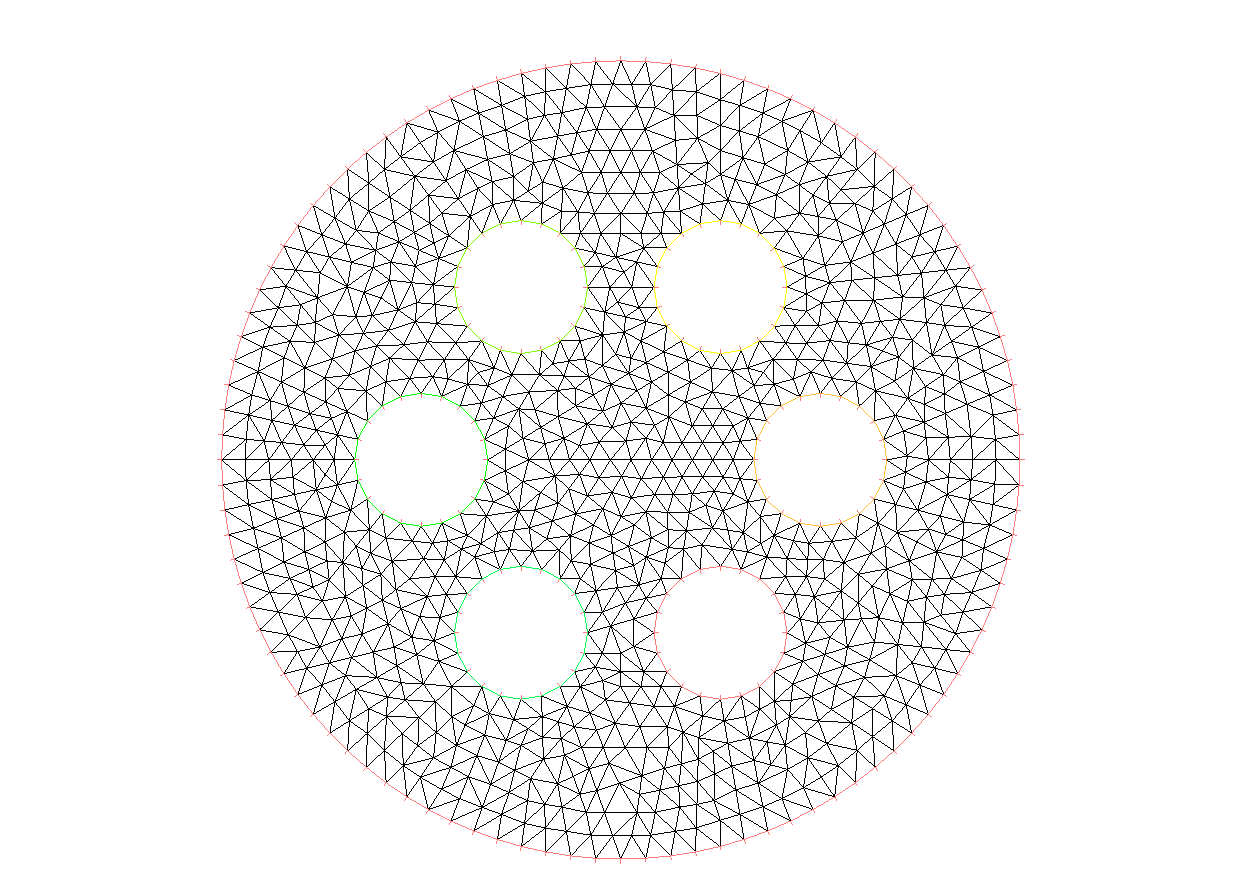
\includegraphics[scale=0.20]{figures/mesh_10.pdf}
  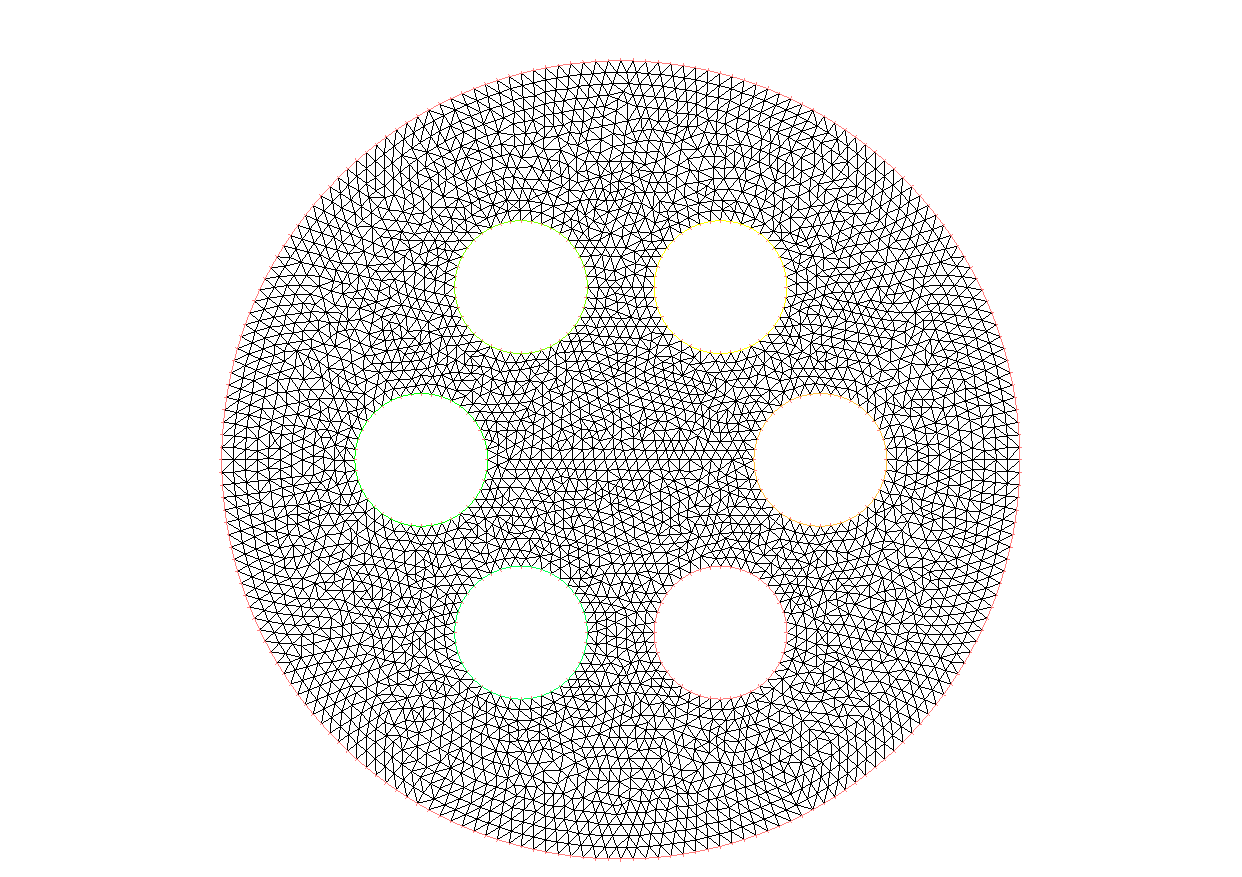
\includegraphics[scale=0.20]{figures/mesh_20.pdf}
  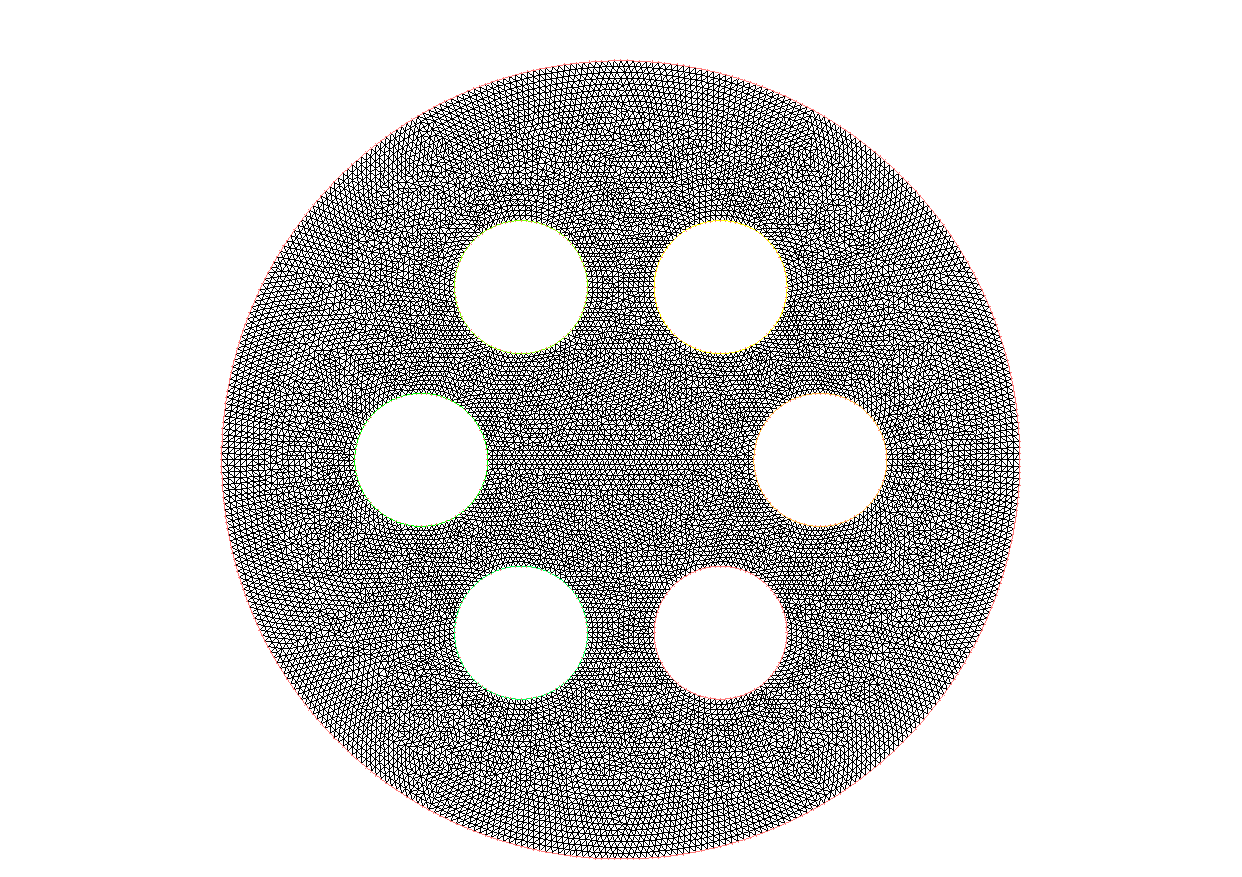
\includegraphics[scale=0.20]{figures/mesh_40.pdf}
  \caption{Mesh family used to compute $M$}
\label{fig:meshfamily}
\end{figure}

The $\zeta_j$ functions are computed on the meshes from fig.
\ref{fig:meshfamily}. For $i \in {1,..,N}$, $\zeta_i$ is determined by solving
the following 

\begin{equation}
  \label{eq:zetapde}
  \begin{array}{rcl}
    -\Delta \zeta_i &=& 0 \quad \text{on }  w_0 \backslash \cup_{k=1}^N \bar{w_k}\\
    \zeta_i &=& \delta_{ij} \quad \text{on } \partial w_j \\ 
  \end{array}  
\end{equation}

as depicted in the figure \ref{fig:zetafamily}.

\begin{figure}[!h]
  \centering
  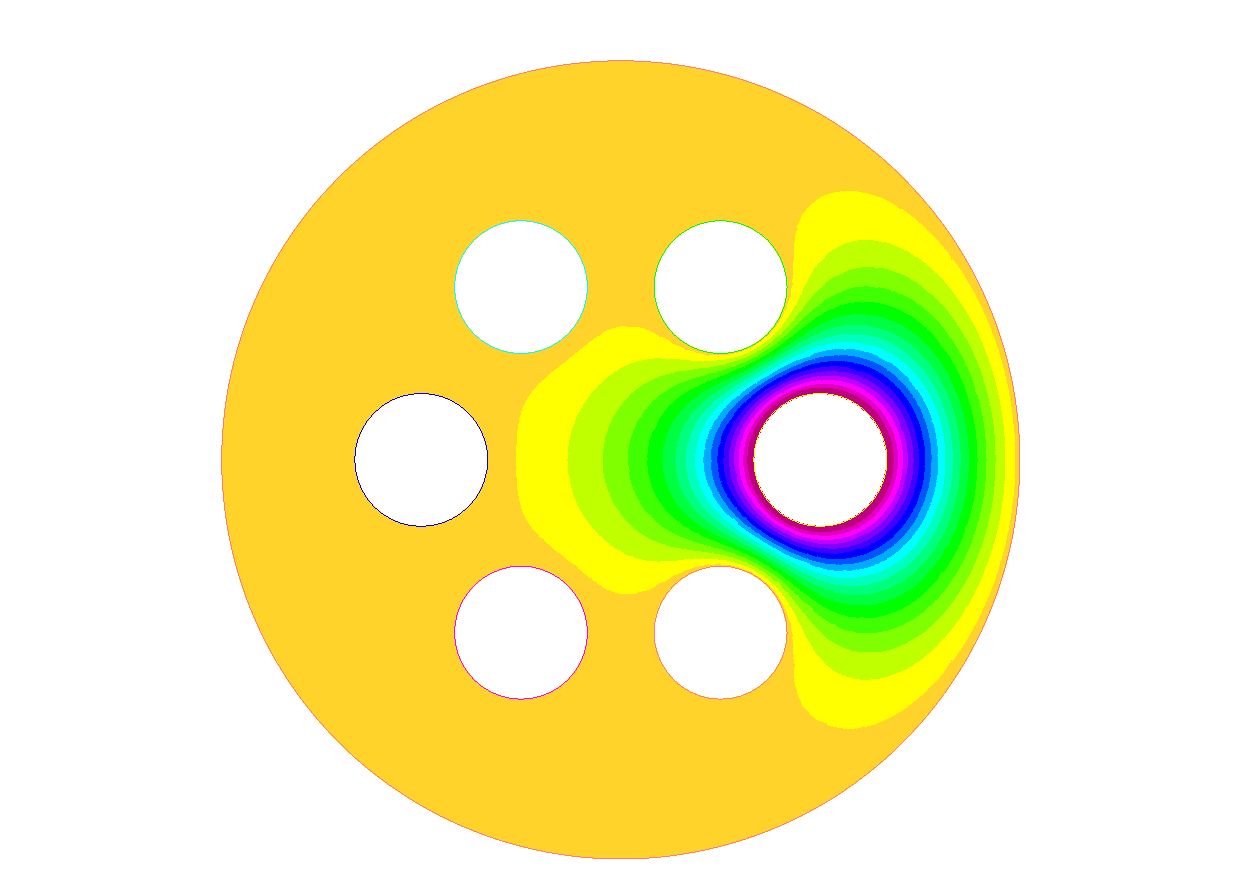
\includegraphics[scale=0.20]{figures/sol_0.pdf}
  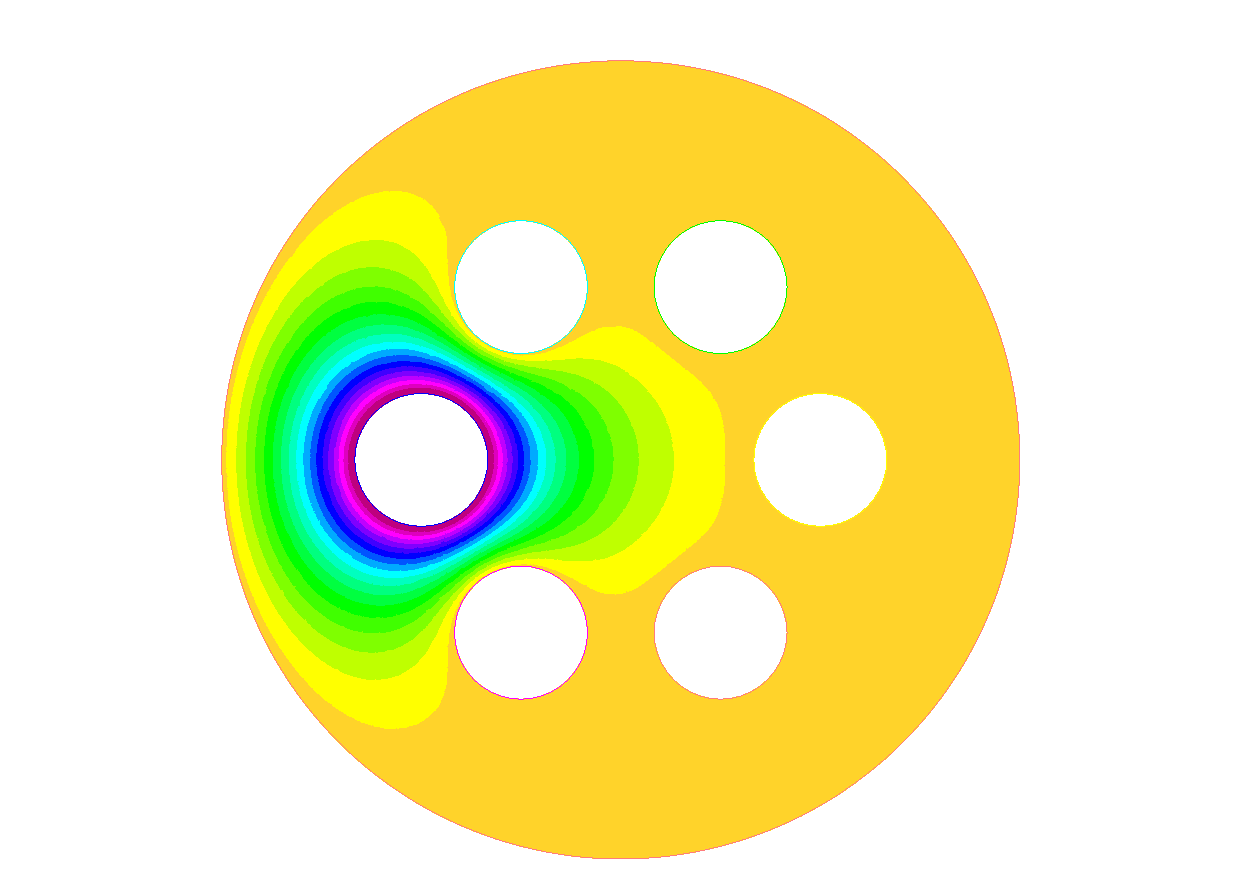
\includegraphics[scale=0.20]{figures/sol_3.pdf}
  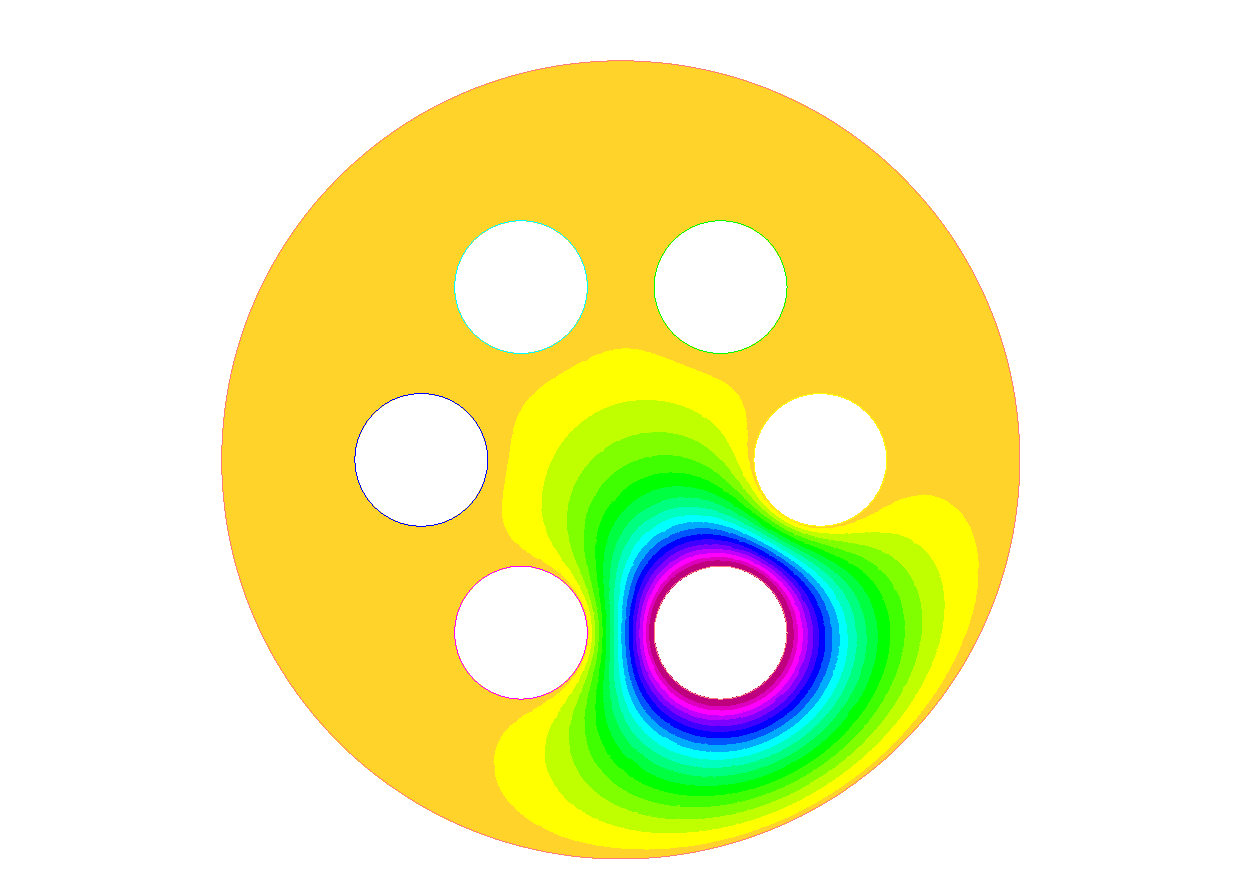
\includegraphics[scale=0.20]{figures/sol_5.pdf}
  \caption{Examples of $\zeta_0,\zeta_3$ and $\zeta_5$}
\label{fig:zetafamily}
\end{figure}


Since the coefficients $M_{ij}$ are computed according to a line integral, we
first test the lack of symmetry versus the smallness \todo{a ameliorer} of the
meshsize. For this, we used the finite element interface FreeFem++ to compute
the desired quantities. The vector space of discrete solutions is based on a
$\mathbb{P}^1$ approximation. The line integral involved in $M_{ij}$ as been
computed with the built-in FreeFem++ command \texttt{int1d(Th,i)(...)}. 

The lack of symmetry is measured by estimating $|| M-M^T ||_\infty$. The
following figure describe the evolution of the error when the mesh size is
decreasing.
\begin{figure}[h]
  \centering
  \begin{tikzpicture}
    \pgfplotsset{width=0.95\textwidth, height=0.4\textwidth}
    \begin{semilogyaxis}[
      ymin=0,
      ymajorgrids=true, % grid=minor pour avoir tous les traits
      xlabel={Mesh size},
      ylabel={$|| M-M^T ||_{\infty}$},
      legend entries={
        Symmetry lack
      },
      legend style={legend pos=north east}
      ]
      \addplot [cyan,thick] table [x index=0,y index=1] {dat/stats_M_simple_case.dat};
      \end{semilogyaxis}
  \end{tikzpicture}
  \caption{Lack of Symmetry vs mesh size}
\label{fig:symm}
\end{figure}


\begin{figure}[h]
  \centering
  \begin{tikzpicture}
    \pgfplotsset{width=0.95\textwidth, height=0.4\textwidth}
    \begin{axis}[
      ymajorgrids=true, % grid=minor pour avoir tous les traits
      xlabel={Mesh size},
      ylabel={cond($M$)},
      legend entries={
        cond(M)
      },
      legend style={legend pos=north east}
      ]
      \addplot [red,thick] table [x index=0,y index=3] {dat/stats_M_simple_case.dat};
      \end{axis}
  \end{tikzpicture}
  \caption{Condition number vs mesh size}
\label{fig:cond}
\end{figure}

\begin{figure}[h]
  \centering
  \begin{tikzpicture}
    \pgfplotsset{width=0.95\textwidth, height=0.2\textwidth}
    \begin{axis}[
      ymajorgrids=true, % grid=minor pour avoir tous les traits
      xlabel={Mesh size},
      ylabel={Smallest eigenvalue},
      legend entries={
        $\lambda_{\text{min}}$
      },
      legend style={legend pos=north east}
      ]
      \addplot [violet,thick] table [x index=0,y index=2] {dat/stats_M_simple_case.dat};
      \end{axis}
  \end{tikzpicture}
  \caption{Smallest eigenvalue vs mesh size}
\label{fig:cond}
\end{figure}
 
The definite positiveness is also verified by the sign of the smallest eigen
value of $M$, we gathered the datum in the following table.

\subsection*{The multiple armour/cable case}
\todo[inline]{rewrite from helluy's doc all the blabla}

\subsection*{Symmetry enforcement by weak formulation}


%%% Local Variables:
%%% mode: latex
%%% TeX-master: "../report"
%%% End:
